\hypertarget{libphonefirewall_8h}{
\section{libphonefirewall.h File Reference}
\label{libphonefirewall_8h}\index{libphonefirewall.h@{libphonefirewall.h}}
}
API of the phone firewall. 



This graph shows which files directly or indirectly include this file:\nopagebreak
\begin{figure}[H]
\begin{center}
\leavevmode
\includegraphics[width=104pt]{libphonefirewall_8h__dep__incl}
\end{center}
\end{figure}
\subsection*{Data Structures}
\begin{CompactItemize}
\item 
struct \hyperlink{structBlacklist}{Blacklist}
\begin{CompactList}\small\item\em Contains the blocked numbers. \item\end{CompactList}\item 
struct \hyperlink{structWhitelist}{Whitelist}
\begin{CompactList}\small\item\em Contains the accepted numbers. \item\end{CompactList}\end{CompactItemize}
\subsection*{Defines}
\begin{CompactItemize}
\item 
\#define \hyperlink{libphonefirewall_8h_b962621ea0404e5dd3d54b4c39cab1a8}{TELNR\_\-MAXLEN}~32
\end{CompactItemize}
\subsection*{Functions}
\begin{CompactItemize}
\item 
int \hyperlink{libphonefirewall_8h_23f18831c9677c1a3b7f8cb6b20f3e02}{add\_\-blacklist\_\-entry} (long long int number, char $\ast$name, char $\ast$reason, int priority)
\item 
int \hyperlink{libphonefirewall_8h_c1875490cf592d507798a292f8a772e9}{rm\_\-blacklist\_\-entry} (long long int number)
\item 
int \hyperlink{libphonefirewall_8h_2f8998691bfe087c701006c9efd2a6cd}{add\_\-whitelist\_\-entry} (long long int number, char $\ast$name, char $\ast$reason, int priority)
\item 
int \hyperlink{libphonefirewall_8h_c3a77117dbcade02ab233836e559814a}{rm\_\-whitelist\_\-entry} (long long int number)
\end{CompactItemize}


\subsection{Detailed Description}
API of the phone firewall. 

\begin{Desc}
\item[Author:]Alex Oberhauser\end{Desc}
The header file of the Phone Firewall. Blocks or accepts incoming phone calls, so it's possible to prevent disturbing phone calls. Provides a API which can used by other application to build nice programs.

Implemented for the OpenMoko framework. 

Definition in file \hyperlink{libphonefirewall_8h-source}{libphonefirewall.h}.

\subsection{Define Documentation}
\hypertarget{libphonefirewall_8h_b962621ea0404e5dd3d54b4c39cab1a8}{
\index{libphonefirewall.h@{libphonefirewall.h}!TELNR\_\-MAXLEN@{TELNR\_\-MAXLEN}}
\index{TELNR\_\-MAXLEN@{TELNR\_\-MAXLEN}!libphonefirewall.h@{libphonefirewall.h}}
\subsubsection{\setlength{\rightskip}{0pt plus 5cm}\#define TELNR\_\-MAXLEN~32}}
\label{libphonefirewall_8h_b962621ea0404e5dd3d54b4c39cab1a8}


The maximum length of a telephone number. 

Definition at line 36 of file libphonefirewall.h.

\subsection{Function Documentation}
\hypertarget{libphonefirewall_8h_23f18831c9677c1a3b7f8cb6b20f3e02}{
\index{libphonefirewall.h@{libphonefirewall.h}!add\_\-blacklist\_\-entry@{add\_\-blacklist\_\-entry}}
\index{add\_\-blacklist\_\-entry@{add\_\-blacklist\_\-entry}!libphonefirewall.h@{libphonefirewall.h}}
\subsubsection{\setlength{\rightskip}{0pt plus 5cm}int add\_\-blacklist\_\-entry (long long int {\em number}, char $\ast$ {\em name}, char $\ast$ {\em reason}, int {\em priority})}}
\label{libphonefirewall_8h_23f18831c9677c1a3b7f8cb6b20f3e02}


Add a number to the blacklist. The number will be blocked after that.

\begin{Desc}
\item[Parameters:]
\begin{description}
\item[{\em number}]The telephone number of the person. \item[{\em name}]The name of the person. \item[{\em reason}]Why you have blocked this person. \item[{\em priority}]Has no affect at the moment. Later one it will be possible to give each number priority. So you have more control when a number will be blocked/accepted.\end{description}
\end{Desc}
\begin{Desc}
\item[Returns:]If all goes well 0 (zero) otherwise an errno code. \end{Desc}


Definition at line 66 of file phonefirewall\_\-administration.c.

References add\_\-to\_\-blacklist().

Here is the call graph for this function:\nopagebreak
\begin{figure}[H]
\begin{center}
\leavevmode
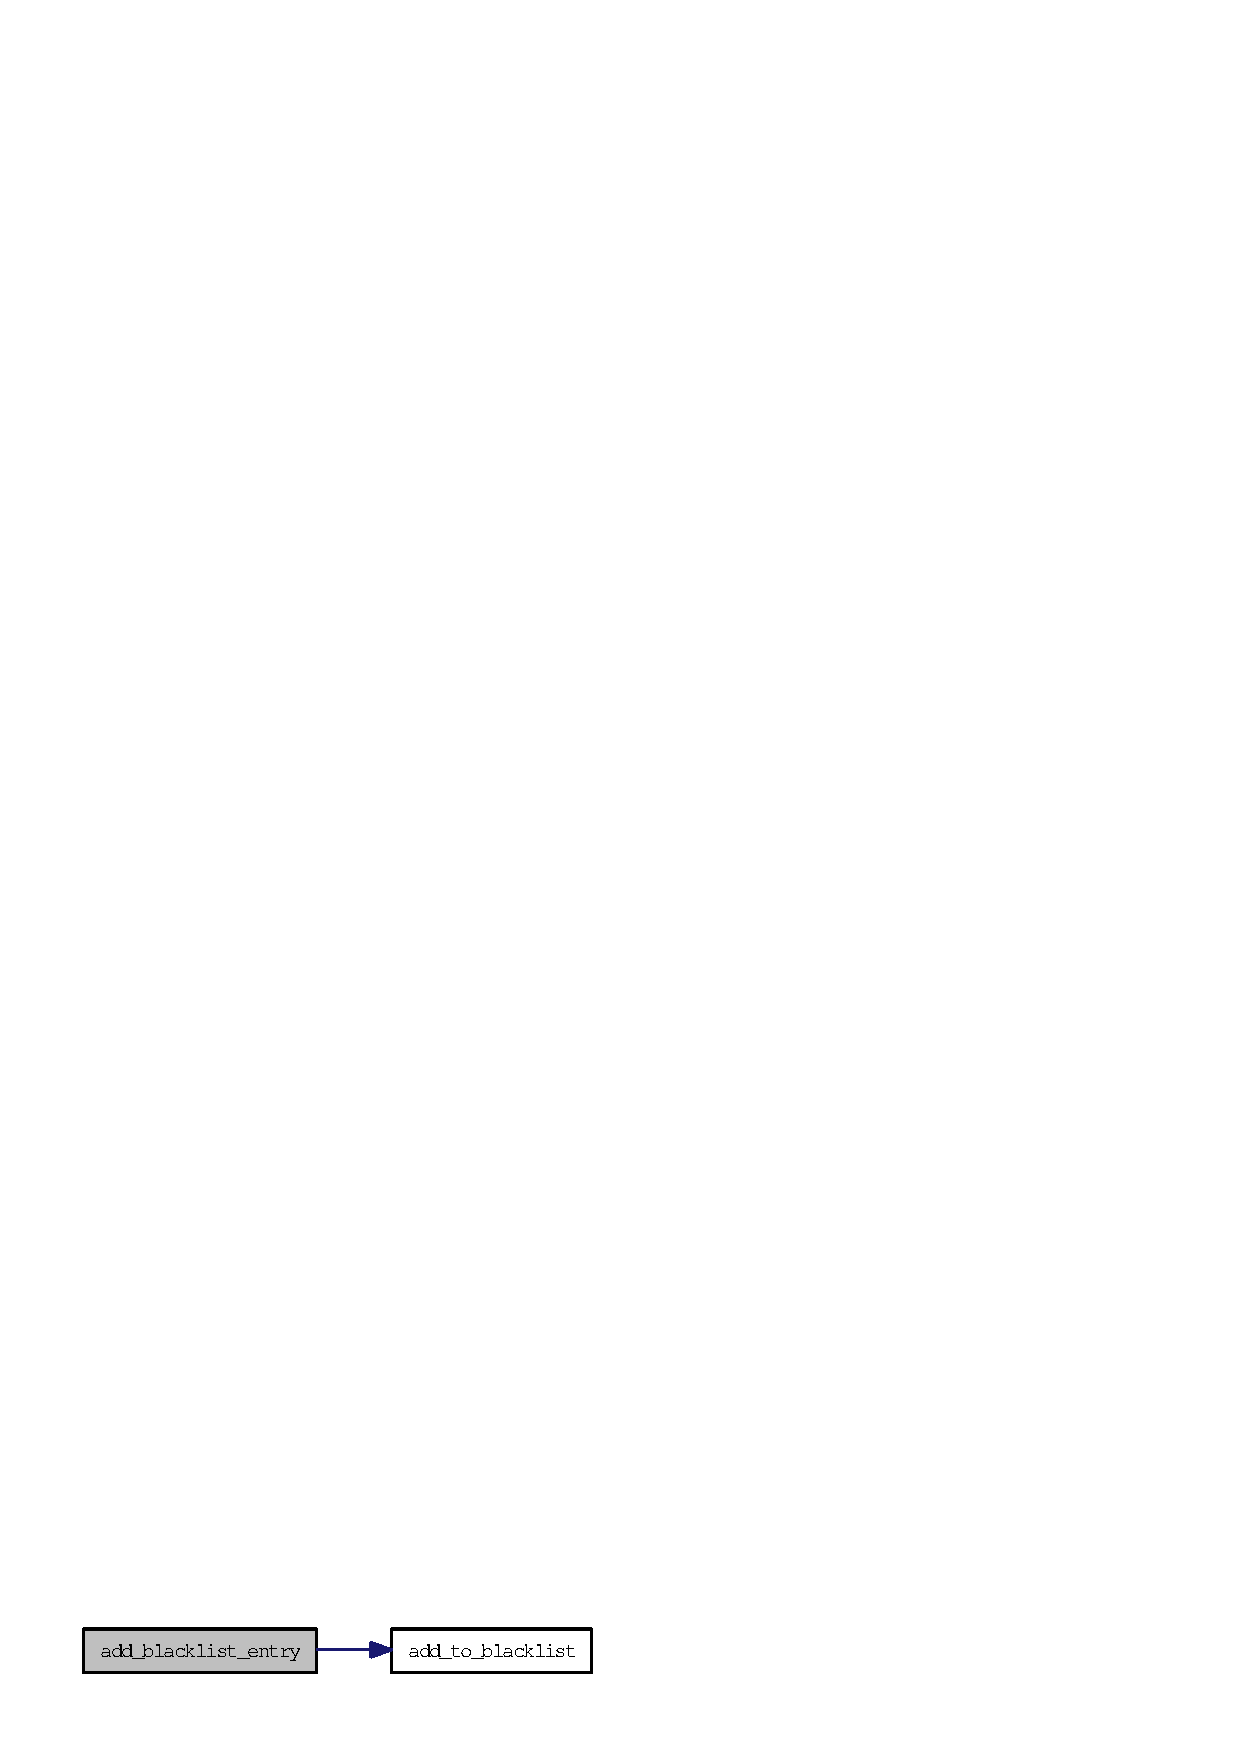
\includegraphics[width=144pt]{libphonefirewall_8h_23f18831c9677c1a3b7f8cb6b20f3e02_cgraph}
\end{center}
\end{figure}
\hypertarget{libphonefirewall_8h_2f8998691bfe087c701006c9efd2a6cd}{
\index{libphonefirewall.h@{libphonefirewall.h}!add\_\-whitelist\_\-entry@{add\_\-whitelist\_\-entry}}
\index{add\_\-whitelist\_\-entry@{add\_\-whitelist\_\-entry}!libphonefirewall.h@{libphonefirewall.h}}
\subsubsection{\setlength{\rightskip}{0pt plus 5cm}int add\_\-whitelist\_\-entry (long long int {\em number}, char $\ast$ {\em name}, char $\ast$ {\em reason}, int {\em priority})}}
\label{libphonefirewall_8h_2f8998691bfe087c701006c9efd2a6cd}


Add a number to the whitelist. The number will be accepted after that.

\begin{Desc}
\item[Parameters:]
\begin{description}
\item[{\em number}]The telephone number of the person. \item[{\em name}]The name of the person. \item[{\em reason}]Why you have blocked this person. \item[{\em priority}]Has no affect at the moment. Later one it will be possible to give each number priority. So you have more control when a number will be blocked/accepted.\end{description}
\end{Desc}
\begin{Desc}
\item[Returns:]If all goes well 0 (zero) otherwise an errno code. \end{Desc}


Definition at line 78 of file phonefirewall\_\-administration.c.\hypertarget{libphonefirewall_8h_c1875490cf592d507798a292f8a772e9}{
\index{libphonefirewall.h@{libphonefirewall.h}!rm\_\-blacklist\_\-entry@{rm\_\-blacklist\_\-entry}}
\index{rm\_\-blacklist\_\-entry@{rm\_\-blacklist\_\-entry}!libphonefirewall.h@{libphonefirewall.h}}
\subsubsection{\setlength{\rightskip}{0pt plus 5cm}int rm\_\-blacklist\_\-entry (long long int {\em number})}}
\label{libphonefirewall_8h_c1875490cf592d507798a292f8a772e9}


Removes a blocked number from the blacklist. 

Definition at line 74 of file phonefirewall\_\-administration.c.\hypertarget{libphonefirewall_8h_c3a77117dbcade02ab233836e559814a}{
\index{libphonefirewall.h@{libphonefirewall.h}!rm\_\-whitelist\_\-entry@{rm\_\-whitelist\_\-entry}}
\index{rm\_\-whitelist\_\-entry@{rm\_\-whitelist\_\-entry}!libphonefirewall.h@{libphonefirewall.h}}
\subsubsection{\setlength{\rightskip}{0pt plus 5cm}int rm\_\-whitelist\_\-entry (long long int {\em number})}}
\label{libphonefirewall_8h_c3a77117dbcade02ab233836e559814a}


Removes a accepted number from the whitelist. 

Definition at line 82 of file phonefirewall\_\-administration.c.